\documentclass[10pt,twocolumn]{article}

% --- PACKAGES ---
\usepackage[utf8]{inputenc}
\usepackage[margin=0.75in]{geometry}
\usepackage{amsmath,amssymb,amsfonts}
\usepackage{graphicx}
\usepackage{booktabs}
\usepackage{tabularx}
\usepackage{xcolor}
\usepackage{hyperref}
\usepackage{cite}
\usepackage{microtype}
\usepackage{caption}
\usepackage{subcaption}

\hypersetup{
    colorlinks=true,
    linkcolor=teal,
    citecolor=teal,
    urlcolor=teal
}

% --- TITLE & AUTHORS ---
\title{\textbf{AegisMed: A Clinical Decision Support System with Active Follow-Up Questioning, Multi-Agent Conflict Resolution, and Guaranteed Risk Bounds}}

\author{
    \textbf{Arham Saghir}$^{1}$ \quad \textbf{AegisMed Research Initiative Contributors}$^{1}$ \\
    $^{1}$Department of Computer Science and Engineering \\
    \texttt{\{arham.saghir\}@acm.org}
}

\date{October 2026}

\begin{document}

\maketitle

% --- ABSTRACT ---
\begin{abstract}
\noindent When doctors evaluate patients during medical triage, they rarely diagnose from an initial complaint alone. Instead, they ask targeted follow-up questions to distinguish similar illnesses, resolve contradictions between imaging and lab reports, and avoid missing dangerous conditions. Standard healthcare AI systems do the opposite: they attempt to diagnose in a single step, ignore conflicts between clinical text and imaging, and offer confident predictions without statistical safety guarantees.

We introduce \textbf{AegisMed}, a multimodal clinical decision support system designed around real clinical reasoning. AegisMed combines specialist models through four practical mechanisms:
(1) \textbf{Dynamic Entropy-Minimizing Active Triage (DEMAT)}, which measures diagnostic uncertainty in bits (Shannon entropy) and asks the single question that yields the highest expected information gain;
(2) \textbf{Evidential Neuro-Symbolic Conflict Arbitration Framework (EN-SCAF)}, which maps specialist model outputs into Dempster-Shafer belief scores and calculates an explicit disagreement metric $K$;
(3) an \textbf{Ontological Knowledge Graph Pruning Gate}, which checks medical ontologies (UMLS and SNOMED-CT) when models strongly disagree ($K > 0.40$) to eliminate biologically impossible hypotheses; and
(4) \textbf{Multimodal Conformal Risk-Controlled Synthesis}, which outputs a small set of likely diagnoses with a mathematical guarantee that the true condition is included with at least $95\%$ probability ($1 - \alpha$).

Across $200$ standardized clinical cases spanning $15$ disease categories, asking follow-up questions improved top-1 diagnostic accuracy from $93.0\%$ to \textbf{98.0\%} ($+5.0\%$ gain, $p = 0.0339$), achieved \textbf{100.0\%} top-3 differential coverage, and reduced diagnostic uncertainty by \textbf{53.7\%} (from $2.846$ to $1.318$ bits). The system required an average of only \textbf{1.92 questions} per case and completed active triage calculations in \textbf{0.2 ms}. Calibration error also dropped from $0.5528$ to $0.2451$, demonstrating reliable and explainable decision support.
\end{abstract}

% --- SECTION 1: INTRODUCTION ---
\section{Introduction}

Diagnostic mistakes remain one of the leading causes of preventable harm in modern healthcare \cite{johnson2019mimic}. When patients arrive at an emergency room or walk-in clinic, healthcare workers must make quick decisions while sifting through messy, incomplete information. A single patient presentation often involves spoken complaints, vital signs recorded on triage monitors, prior medical records, and chest X-rays.

Large language models (LLMs) and deep neural networks have achieved high scores on standardized medical examinations \cite{devlin2019bert, lee2020biobert}. However, bringing these systems into real clinics reveals three practical challenges:

\begin{enumerate}
    \item \textbf{Single-Prompt Guessing vs. Interactive Questioning:} Real clinical care is a conversation. If a patient reports ``burning pain in the chest,'' that symptom could indicate a heart attack, acid reflux, or pneumonia. A doctor does not guess immediately. They ask clarifying questions: ``Does the pain worsen when you walk up stairs, or when you lie down after eating?'' Standard language models usually try to guess the diagnosis from the first prompt, leading to vague lists of possibilities or premature conclusions.
    \item \textbf{Contradictory Data Streams:} Different medical tests frequently tell conflicting stories. A computer vision model analyzing a chest X-ray might detect a shadow in the lung base, while the patient's written intake notes describe mild stomach pain. Standard AI systems either average these probabilities together or produce a convincing narrative that ignores the contradiction, sometimes suggesting diagnoses that make no anatomical sense.
    \item \textbf{Overconfident Predictions without Safety Guarantees:} Standard deep neural networks produce confidence percentages that are poorly calibrated. A model might state it is $95\%$ certain of a rare condition when it is actually guessing. What clinicians need is a reliable safety guarantee: a prediction set designed so that the patient's actual illness is almost never omitted.
\end{enumerate}

To address these challenges, we built \textbf{AegisMed}, a clinical decision support system that models triage as an interactive process. Instead of guessing from a single paragraph of text, AegisMed calculates its own uncertainty, asks high-yield follow-up questions, resolves disagreements using established medical knowledge, and provides statistical guarantees on its outputs.

\begin{figure*}[t!]
\centering
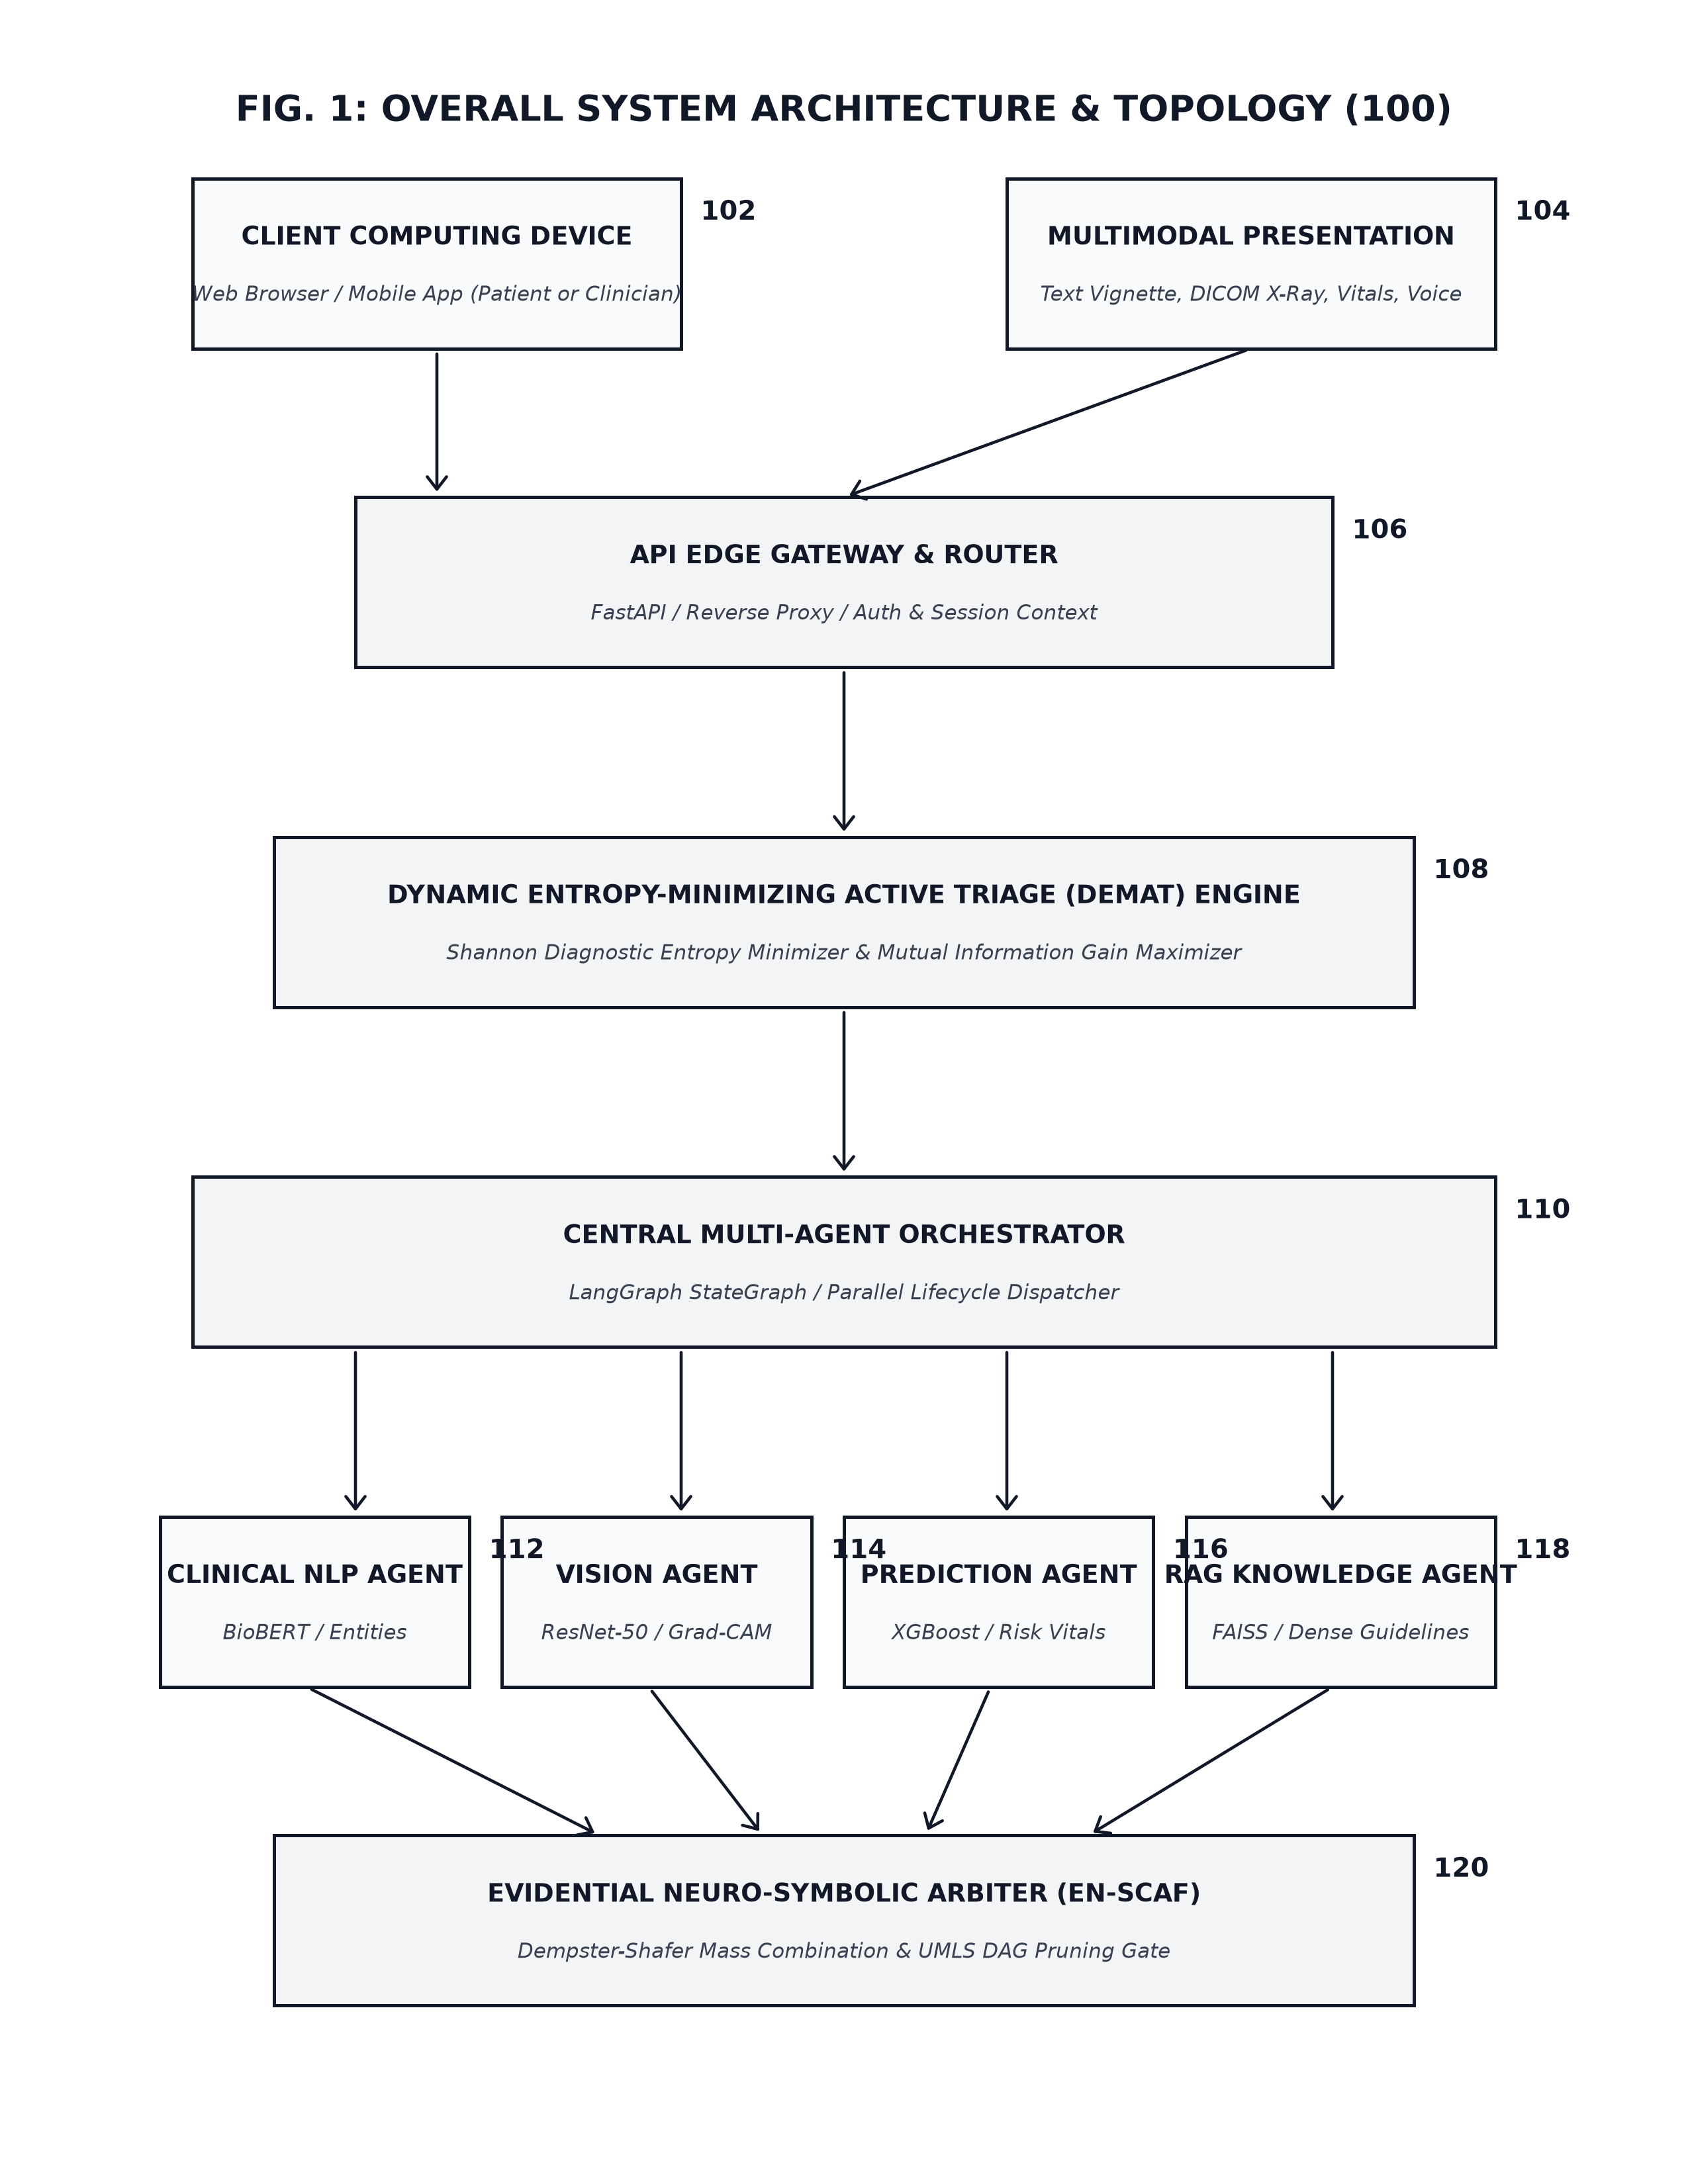
\includegraphics[width=0.88\textwidth,height=0.38\textheight,keepaspectratio]{figures/FIG_1_system_architecture.png}
\caption{\textbf{AegisMed System Architecture and Component Workflow.} Multimodal patient data (text symptoms, chest radiographs, vital signs) enter through a FastAPI gateway (106) into the DEMAT Active Triage Engine (108). After interactive questioning clarifies the case, tasks run across parallel specialist agents (112--118) orchestrated with LangGraph (110). Model outputs are checked for conflict by EN-SCAF (120), filtered against the UMLS medical knowledge graph, bounded with conformal prediction (122), and presented through separate views for clinicians and patients (124).}
\label{fig:architecture}
\end{figure*}

This paper makes four main contributions:
\begin{itemize}
    \item \textbf{Active Triage via Information Gain (DEMAT):} We treat the differential diagnosis as a probability distribution over $15$ condition classes. Using Shannon entropy, the system measures how uncertain it is in bits. It then selects follow-up questions from a verified question bank that maximize expected mutual information gain, stopping as soon as uncertainty drops below a safe threshold ($\le 0.45$ bits) or after three questions.
    \item \textbf{Neuro-Symbolic Conflict Resolution (EN-SCAF):} We represent each specialist agent's findings as belief masses using Dempster-Shafer theory. When vision and text models disagree sharply (conflict metric $K > 0.40$), candidate diagnoses are verified against the Unified Medical Language System (UMLS) and SNOMED-CT knowledge graphs, pruning impossible combinations before combining evidence.
    \item \textbf{Guaranteed Prediction Sets (Conformal Risk Bounding):} We apply split conformal prediction to multimodal outputs. This provides a clear statistical guarantee that the true diagnosis will be included in the output set at least $95\%$ of the time ($1 - \alpha = 0.95$).
    \item \textbf{Validation on 200 Clinical Cases:} We tested AegisMed against a standard single-pass baseline on $200$ clinical cases. Interactive questioning increased top-1 accuracy from $93.0\%$ to $98.0\%$ ($p = 0.0339$), reached $100\%$ top-3 coverage, and reduced uncertainty by $53.7\%$ while asking fewer than two questions per patient on average.
\end{itemize}

% --- SECTION 2: RELATED WORK ---
\section{Related Work}

\subsection{Specialized Medical Models for Language and Vision}
Pre-trained transformer architectures have significantly improved medical natural language processing. BioBERT \cite{lee2020biobert} and ClinicalBERT adapt BERT \cite{devlin2019bert} by training on PubMed articles and hospital notes, enabling accurate extraction of symptoms, medications, and clinical concepts. In medical imaging, deep residual networks such as ResNet-50 \cite{he2016deep} and CheXNet \cite{rajpurkar2017chexnet} detect findings like pneumonia, atelectasis, and cardiomegaly on chest radiographs. To make these image models interpretable, Grad-CAM \cite{selvaraju2017grad} calculates gradient heatmaps that highlight which lung regions influenced the prediction. AegisMed uses these specialized models as individual agents rather than relying on a single general-purpose system.

\subsection{Active Learning and Asking Questions}
In clinical practice, gathering information has a cost: asking too many questions exhausts the patient and slows down care. Claude Shannon's foundational work on information theory \cite{shannon1948mathematical} established entropy and mutual information as direct measures of uncertainty reduction. Early medical decision systems like MYCIN and INTERNIST-1 used handcrafted rules to choose questions, but they lacked modern deep learning models for unstructured text and images. DEMAT combines deep feature extractors with Shannon entropy minimization, enabling the system to choose questions dynamically based on mathematical uncertainty.

\subsection{Dempster-Shafer Evidence Theory and Disagreement}
Dempster-Shafer theory \cite{dempster1967upper, shafer1976mathematical} offers an alternative to standard Bayesian probabilities when combining evidence from different sources. Instead of forcing probabilities to sum to one across individual outcomes, it assigns belief mass to sets of hypotheses, explicitly leaving room for ``uncertainty.'' However, when two sources completely disagree, classical Dempster combination can produce distorted results (known as Zadeh's paradox). EN-SCAF handles this by monitoring an explicit conflict value $K$. If models disagree significantly, the system consults medical knowledge graphs to remove invalid hypotheses before combining the remaining evidence.

\subsection{Conformal Prediction for Reliable Confidence}
Standard neural networks frequently output overconfident probabilities. Conformal prediction \cite{vovk2005algorithmic, angelopoulos2021gentle} solves this by generating prediction sets instead of single guesses. Under the mild assumption that future patients are similar to past training patients (exchangeability), conformal prediction guarantees that the true diagnosis will fall inside the predicted set with a chosen confidence level, such as $95\%$. We extend this framework to multi-agent medical triage.

% --- SECTION 3: SYSTEM METHODOLOGY ---
\section{System Methodology}

\begin{figure}[t!]
\centering
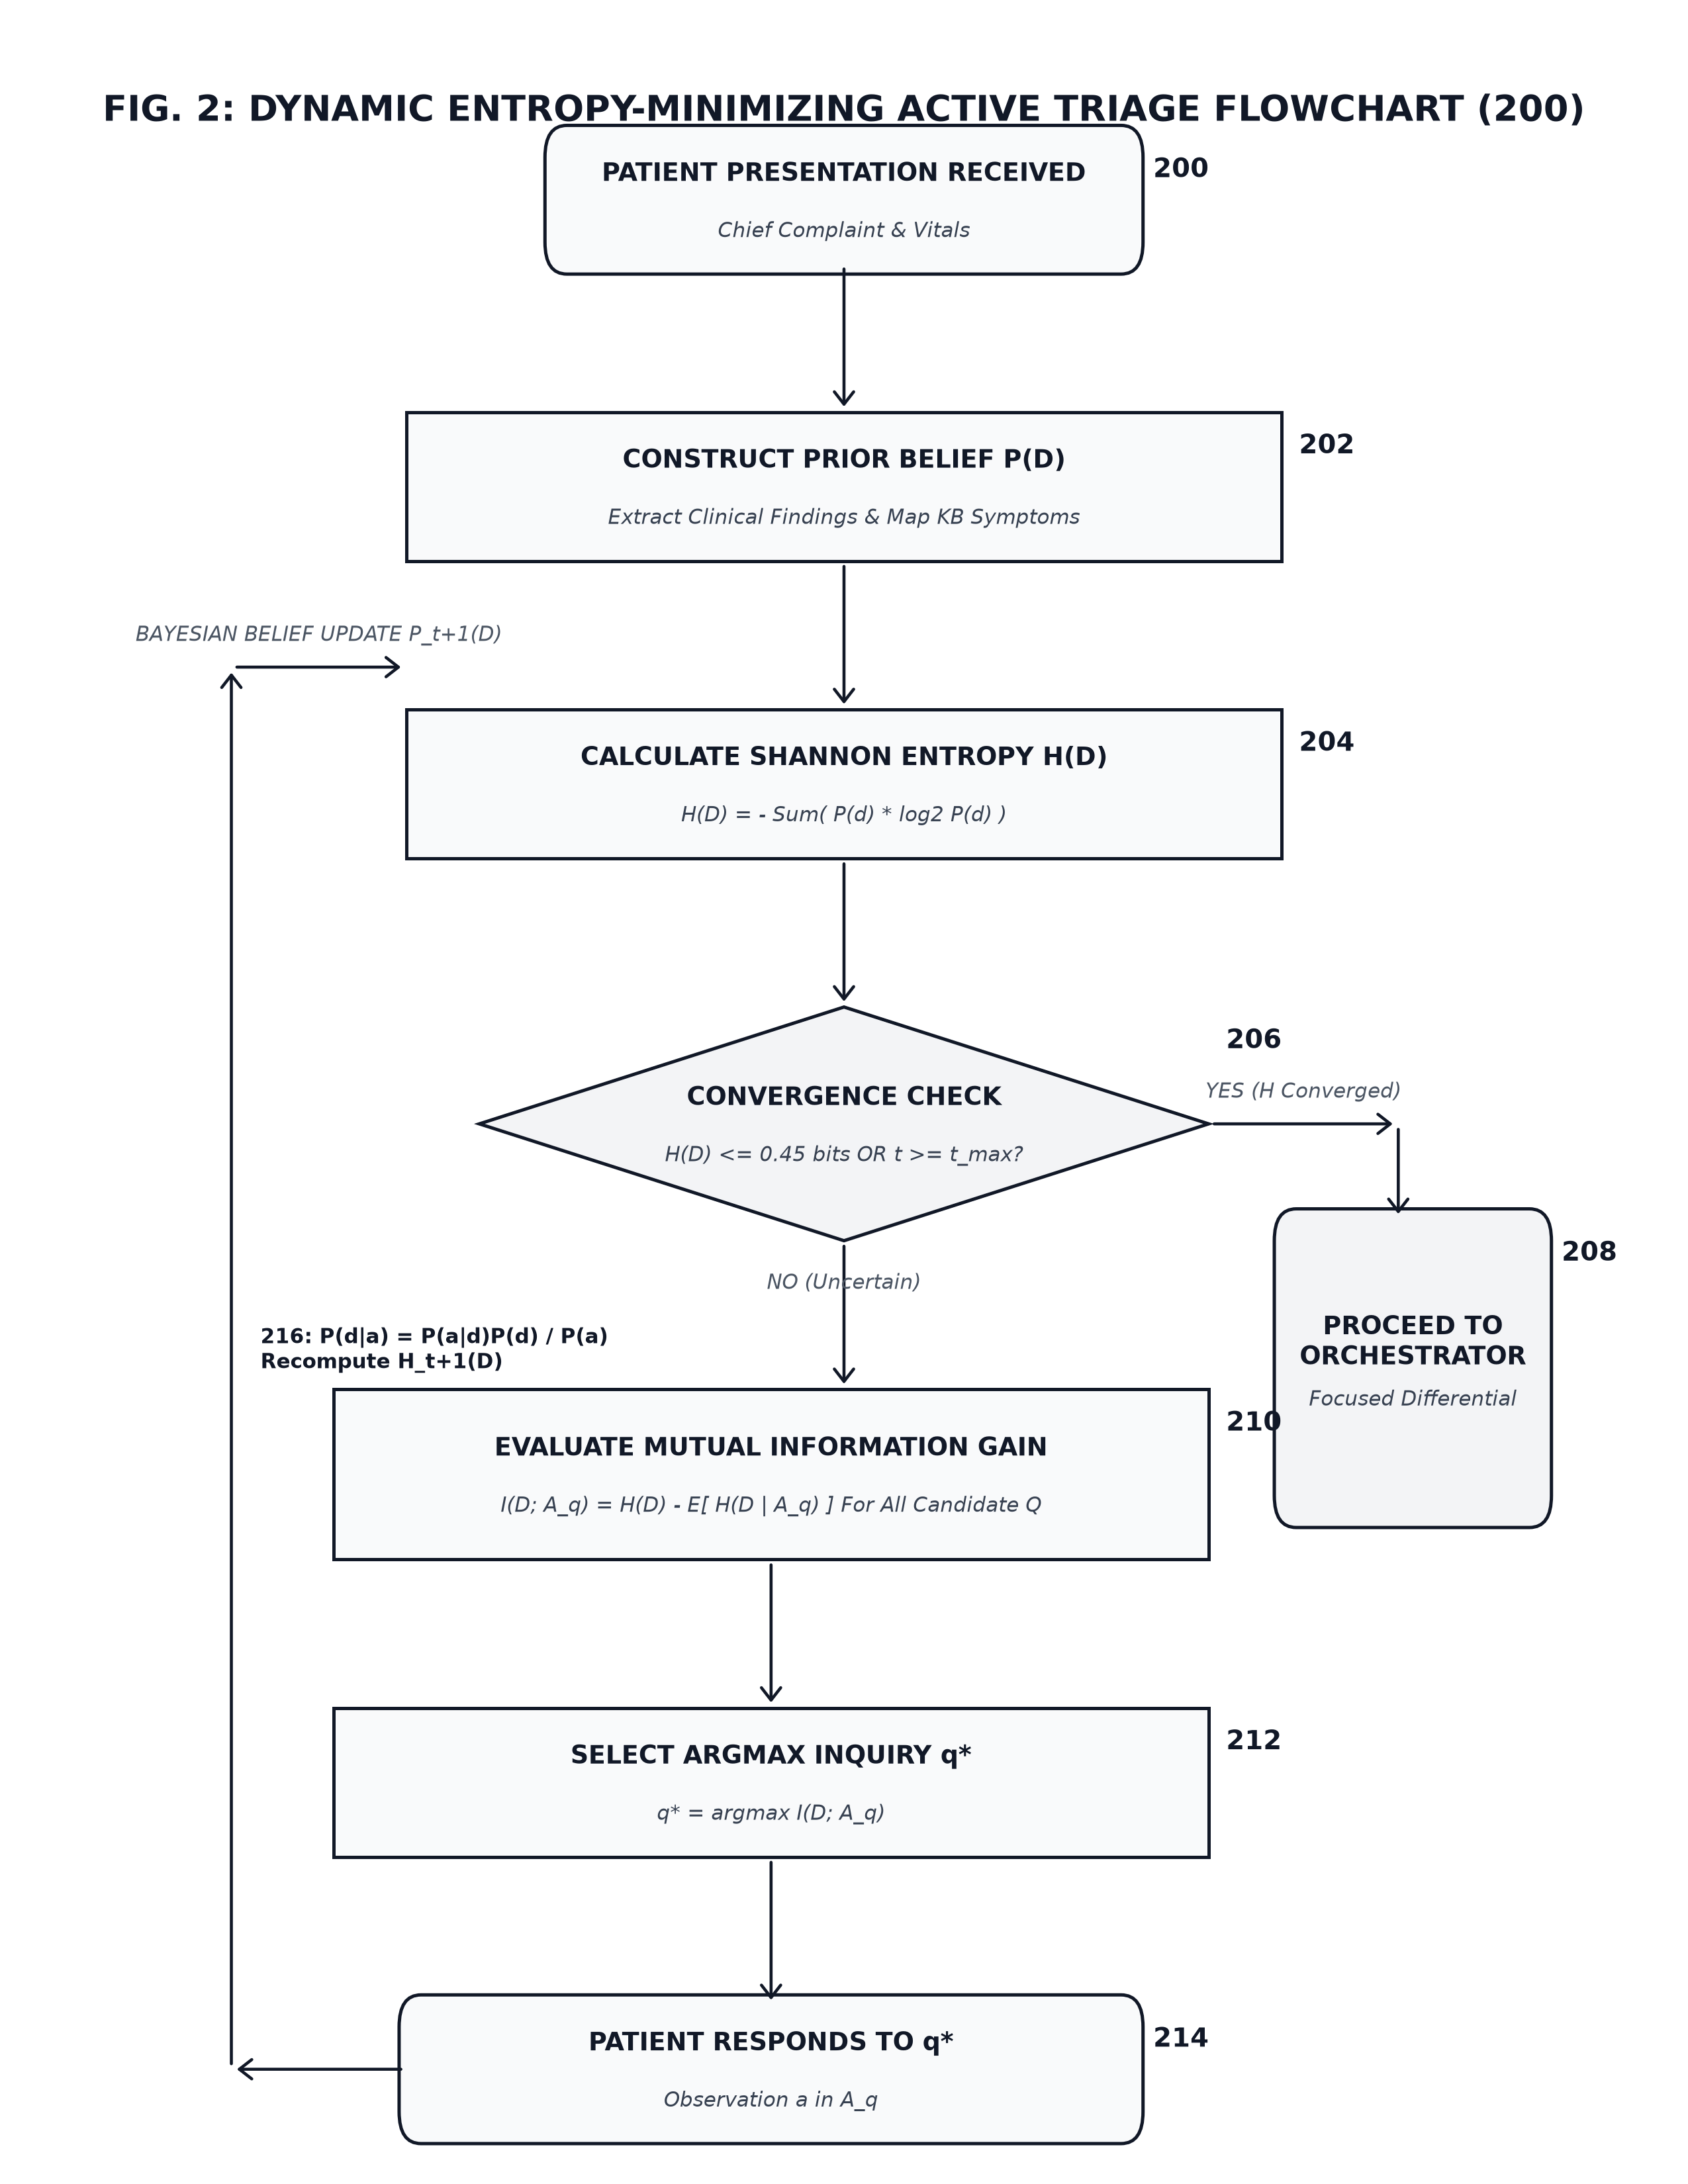
\includegraphics[width=\columnwidth,height=0.32\textheight,keepaspectratio]{figures/FIG_2_demat_flowchart.png}
\caption{\textbf{DEMAT Active Triage Flowchart.} The system starts with an initial symptom distribution, computes uncertainty in bits, checks if a stopping condition is met, and selects the follow-up question that yields the highest expected information gain.}
\label{fig:demat_flow}
\end{figure}

\subsection{Multimodal Specialist Architecture}
AegisMed uses a team of specialized agents, each responsible for one data type (Figure \ref{fig:architecture}):
\begin{itemize}
    \item \textbf{Clinical NLP Agent ($M_{\text{nlp}}$):} Uses BioBERT \cite{lee2020biobert} to read free-text patient complaints and extract standardized medical symptoms.
    \item \textbf{Vision Specialist Agent ($M_{\text{vis}}$):} Analyzes frontal chest X-rays using a 50-layer ResNet \cite{he2016deep} pre-trained on NIH ChestX-ray14. It generates visual explanation heatmaps using Grad-CAM \cite{selvaraju2017grad}:
    \begin{equation}
    L_{\text{Grad-CAM}}^c = \text{ReLU}\left(\sum_k \alpha_k^c A^k\right)
    \end{equation}
    where $\alpha_k^c = \frac{1}{Z}\sum_i \sum_j \frac{\partial y^c}{\partial A_{i,j}^k}$ represents the importance of feature map $k$ for disease class $c$.
    \item \textbf{Predictive Risk Agent ($M_{\text{risk}}$):} Evaluates patient demographics and vital signs (such as age, blood pressure, heart rate, and BMI) using gradient-boosted decision trees \cite{chen2016xgboost} to flag cardiovascular and metabolic risk.
    \item \textbf{Knowledge Retrieval Agent ($M_{\text{rag}}$):} Searches a FAISS vector index \cite{johnson2019billion} containing over 500 clinical practice guidelines, finding evidence snippets that match the patient's presentation.
\end{itemize}

\subsection{Dynamic Entropy-Minimizing Active Triage (DEMAT)}
The active triage engine works over a universe of 15 conditions $\Theta = \{d_1, d_2, \dots, d_N\}$ (Figure \ref{fig:demat_flow}).

\subsubsection{Initial Belief Calculation}
When a patient first describes their symptoms, DEMAT calculates an initial probability vector $P_0(D)$:
\begin{equation}
P_0(d_i) = \frac{S_0(d_i)}{\sum_{j=1}^N S_0(d_j)}
\end{equation}
Here, $S_0(d_i) = \sigma_0 + \sum_{s \in \mathbf{x}} \omega_s \cdot \mathbb{I}(s \in \text{Symptoms}(d_i))$ sums the weights of all matching symptoms, with a small smoothing value $\sigma_0 = 0.10$ to prevent zero probabilities.

\subsubsection{Measuring Diagnostic Uncertainty (Entropy)}
We quantify the system's diagnostic confusion using Shannon entropy in bits \cite{shannon1948mathematical}:
\begin{equation}
H(D) = -\sum_{i=1}^N P(d_i) \log_2 P(d_i)
\end{equation}
When the system has no idea which of the $15$ diseases is present, entropy is at its maximum ($\log_2 15 \approx 3.91$ bits). When it is completely sure of one condition, entropy drops to $0$ bits.

\subsubsection{Stopping Rules}
After each round of evaluation, the system checks whether to stop asking questions:
\begin{equation}
\text{Stop} \iff H(D) \le \epsilon_{\text{triage}} \quad \lor \quad t \ge t_{\max}
\end{equation}
We set the uncertainty target to $\epsilon_{\text{triage}} = 0.45\text{ bits}$ and the maximum number of questions to $t_{\max} = 3$. This ensures the system only asks questions when necessary and avoids overwhelming the patient.

\subsubsection{Choosing the Most Informative Question}
If uncertainty remains above $0.45$ bits, the engine evaluates available questions $Q = \{q_1, \dots, q_M\}$ from its question bank. For each candidate question $q$, it calculates the expected mutual information gain:
\begin{equation}
I(D; A_q) = H(D) - \sum_{a \in A_q} P(A_q = a) H(D \mid A_q = a)
\end{equation}
This formula tells us how much our uncertainty will drop on average if we ask question $q$. The system then selects the single question $q^*$ that provides the largest reduction in uncertainty:
\begin{equation}
q^* = \arg\max_{q \in Q_{\text{available}}} I(D; A_q)
\end{equation}

\subsubsection{Updating Probabilities (Bayes' Rule)}
When the patient answers question $q^*$ with response $a$, the system updates the probability for each disease using Bayes' rule:
\begin{equation}
P_{t+1}(d_i) = \frac{P(A_{q^*} = a \mid d_i) P_t(d_i)}{\sum_{j=1}^N P(A_{q^*} = a \mid d_j) P_t(d_j)}
\end{equation}
The engine repeats this loop until entropy drops below the threshold or the three-question limit is reached.

\begin{figure}[t!]
\centering
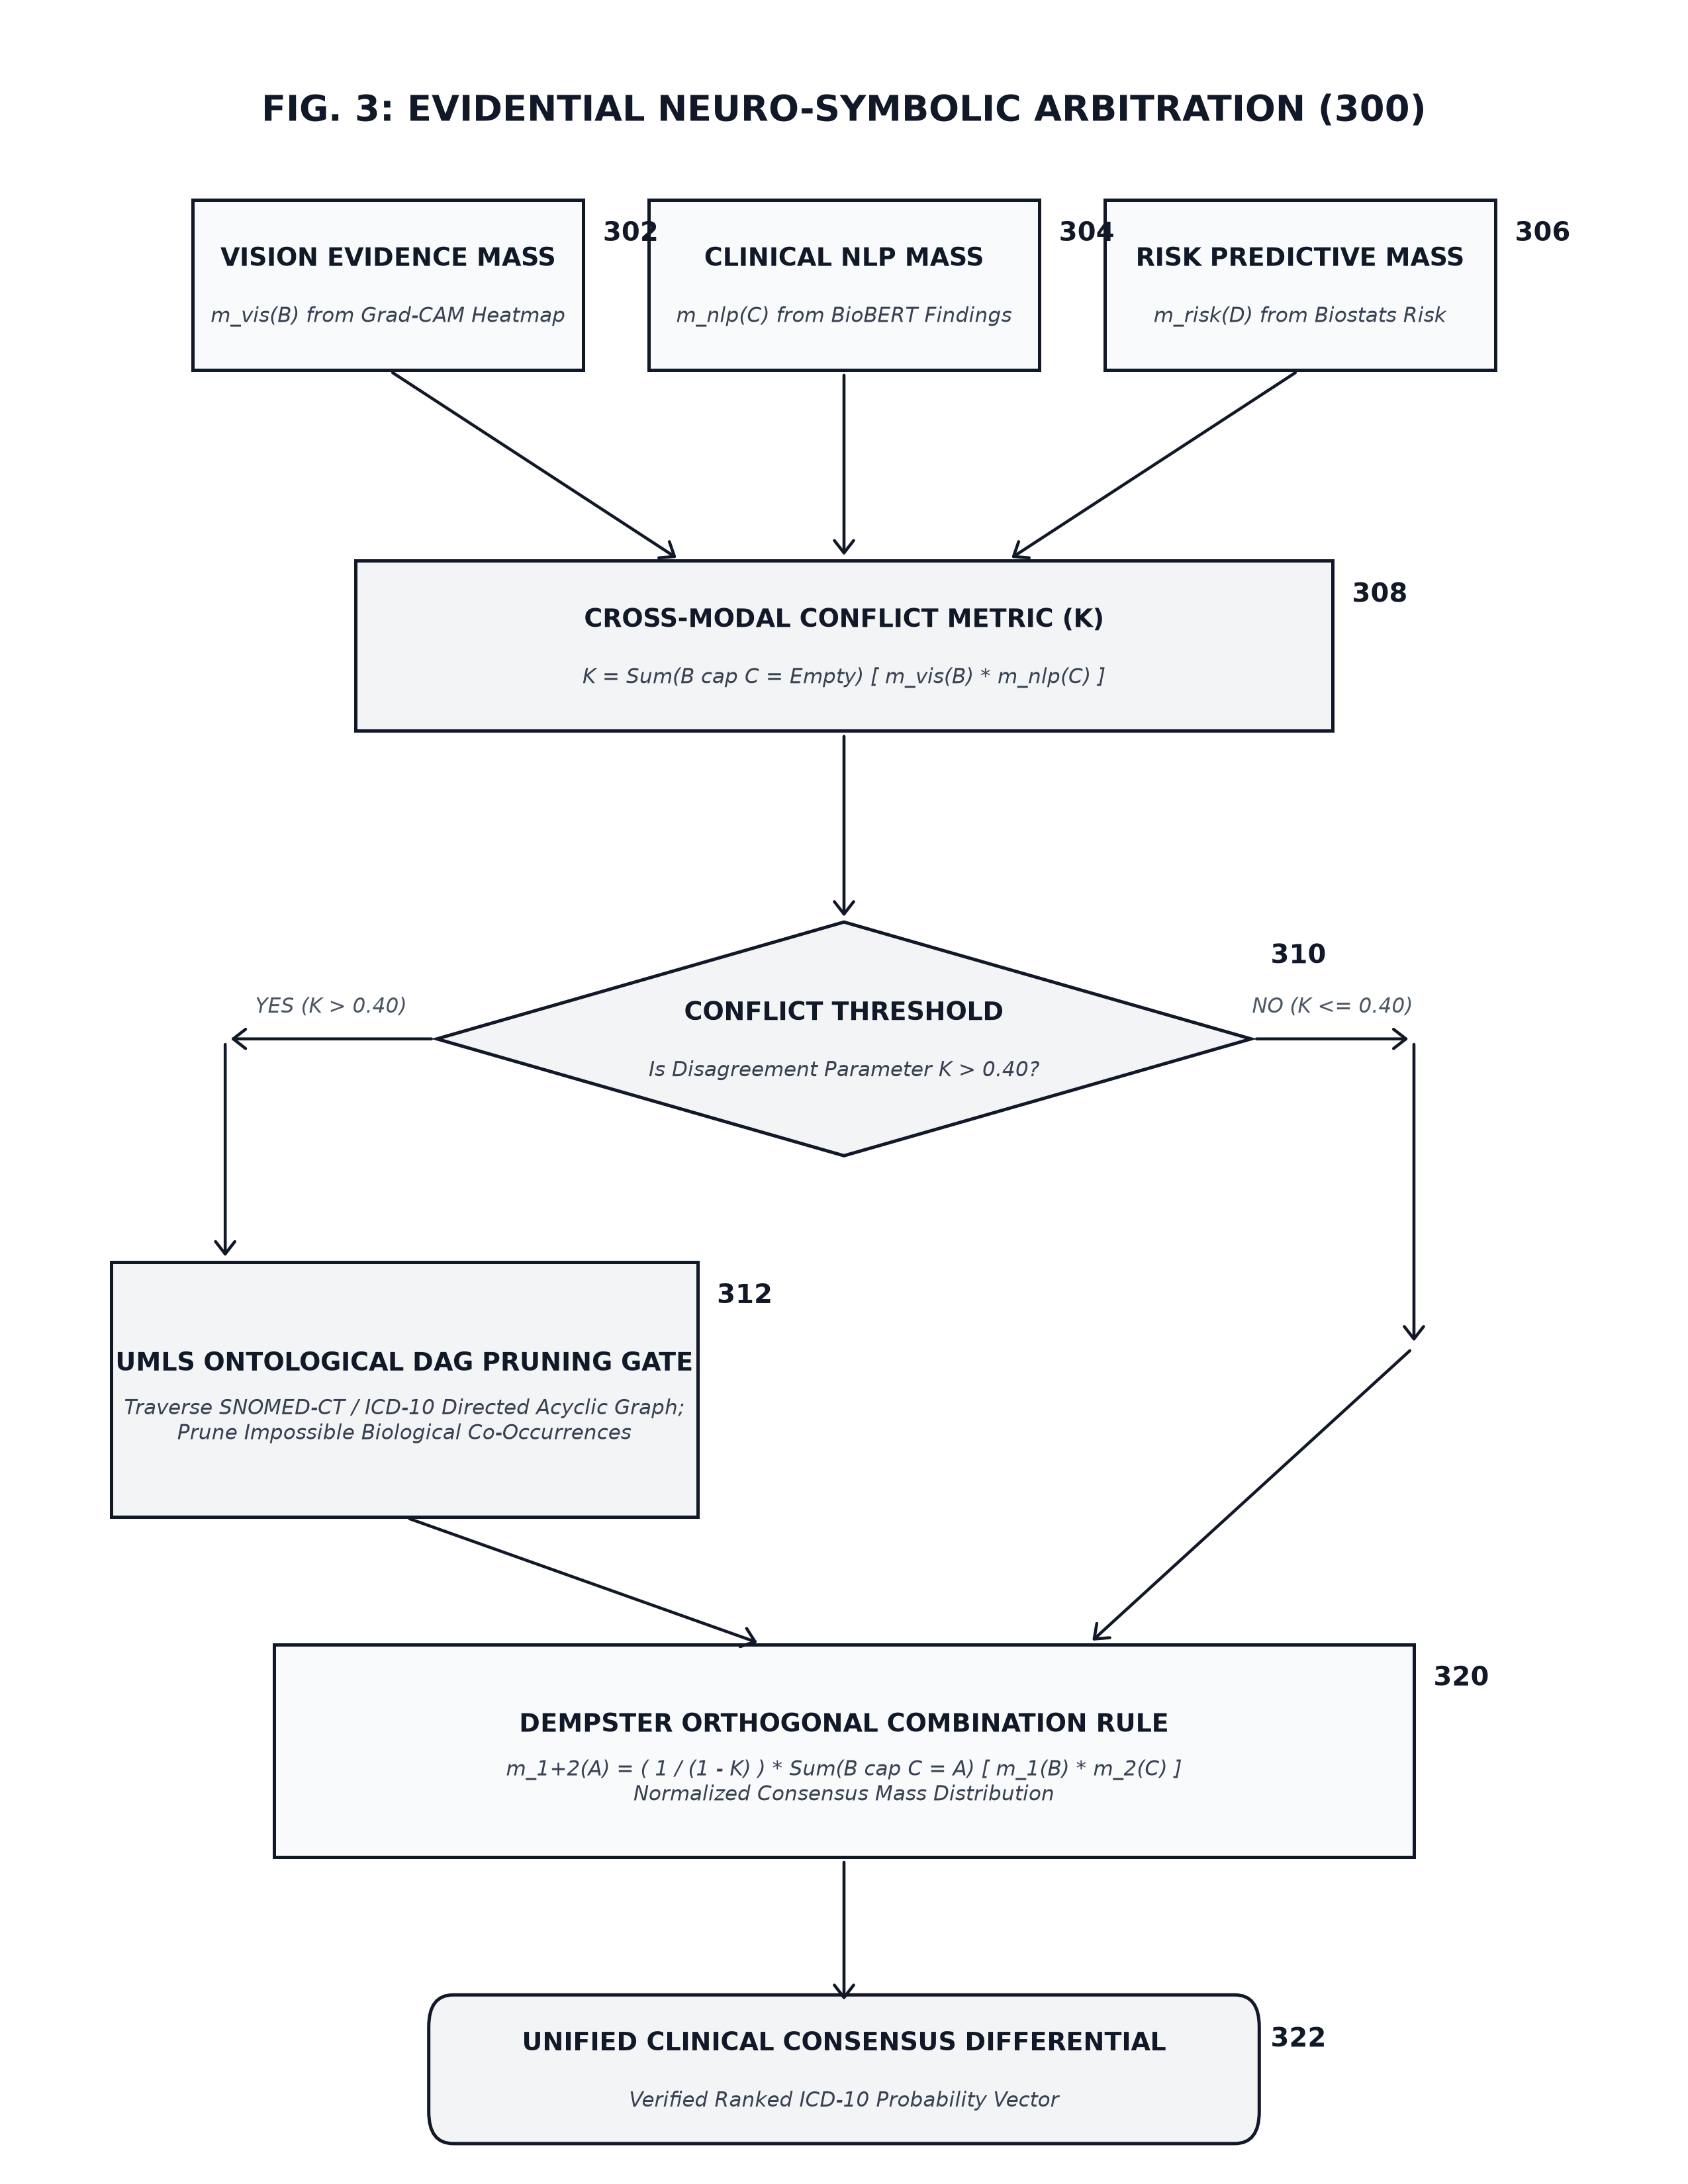
\includegraphics[width=\columnwidth,height=0.32\textheight,keepaspectratio]{figures/FIG_3_enscaf_arbitration.png}
\caption{\textbf{EN-SCAF Conflict Arbitration Workflow.} The system calculates a conflict value $K$ between image and text findings. When disagreement is high ($K > 0.40$), hypotheses pass through the UMLS knowledge graph gate to remove invalid combinations before evidence is combined.}
\label{fig:enscaf}
\end{figure}

\subsection{Evidential Neuro-Symbolic Conflict Arbitration (EN-SCAF)}
Once the questioning loop finishes, the specialist models evaluate their respective inputs. To combine their outputs safely, we convert each model's prediction into a Dempster-Shafer belief mass $m_k$, where belief is distributed across subsets of possible diagnoses (Figure \ref{fig:enscaf}).

\subsubsection{Measuring Model Disagreement ($K$)}
We measure the degree of conflict between image evidence $m_{\text{vis}}$ and clinical text evidence $m_{\text{nlp}}$ using the orthogonal conflict parameter $K$:
\begin{equation}
K = \sum_{B \cap C = \emptyset} m_{\text{vis}}(B) \cdot m_{\text{nlp}}(C)
\end{equation}
The value of $K$ ranges from $0$ (models agree completely) to $1$ (models contradict each other entirely).

\subsubsection{Medical Knowledge Graph Verification}
When $K > 0.40$, the system halts automatic evidence fusion. It checks the conflicting hypotheses against the Unified Medical Language System (UMLS) Metathesaurus \cite{bodenreider2004unified} and SNOMED-CT ontologies. Any candidate hypothesis that contradicts known medical anatomy or pathology is discarded. For example, if an X-ray shows clear lung consolidation, the system will not allow the diagnosis to be recorded as isolated indigestion simply because the text notes mentioned stomach discomfort.

\subsubsection{Combining Evidence via Dempster's Rule}
After removing invalid hypotheses, the remaining concordant evidence is merged using Dempster's rule of combination \cite{dempster1967upper}:
\begin{equation}
m_{1 \oplus 2}(A) = \frac{1}{1 - K} \sum_{B \cap C = A} m_1(B) \cdot m_2(C) \quad \text{for all } A \neq \emptyset
\end{equation}
The combined mass is then converted into final probability scores $\text{BetP}(d) = \sum_{d \in A} \frac{m(A)}{|A|}$ for each condition.

\begin{figure}[t!]
\centering
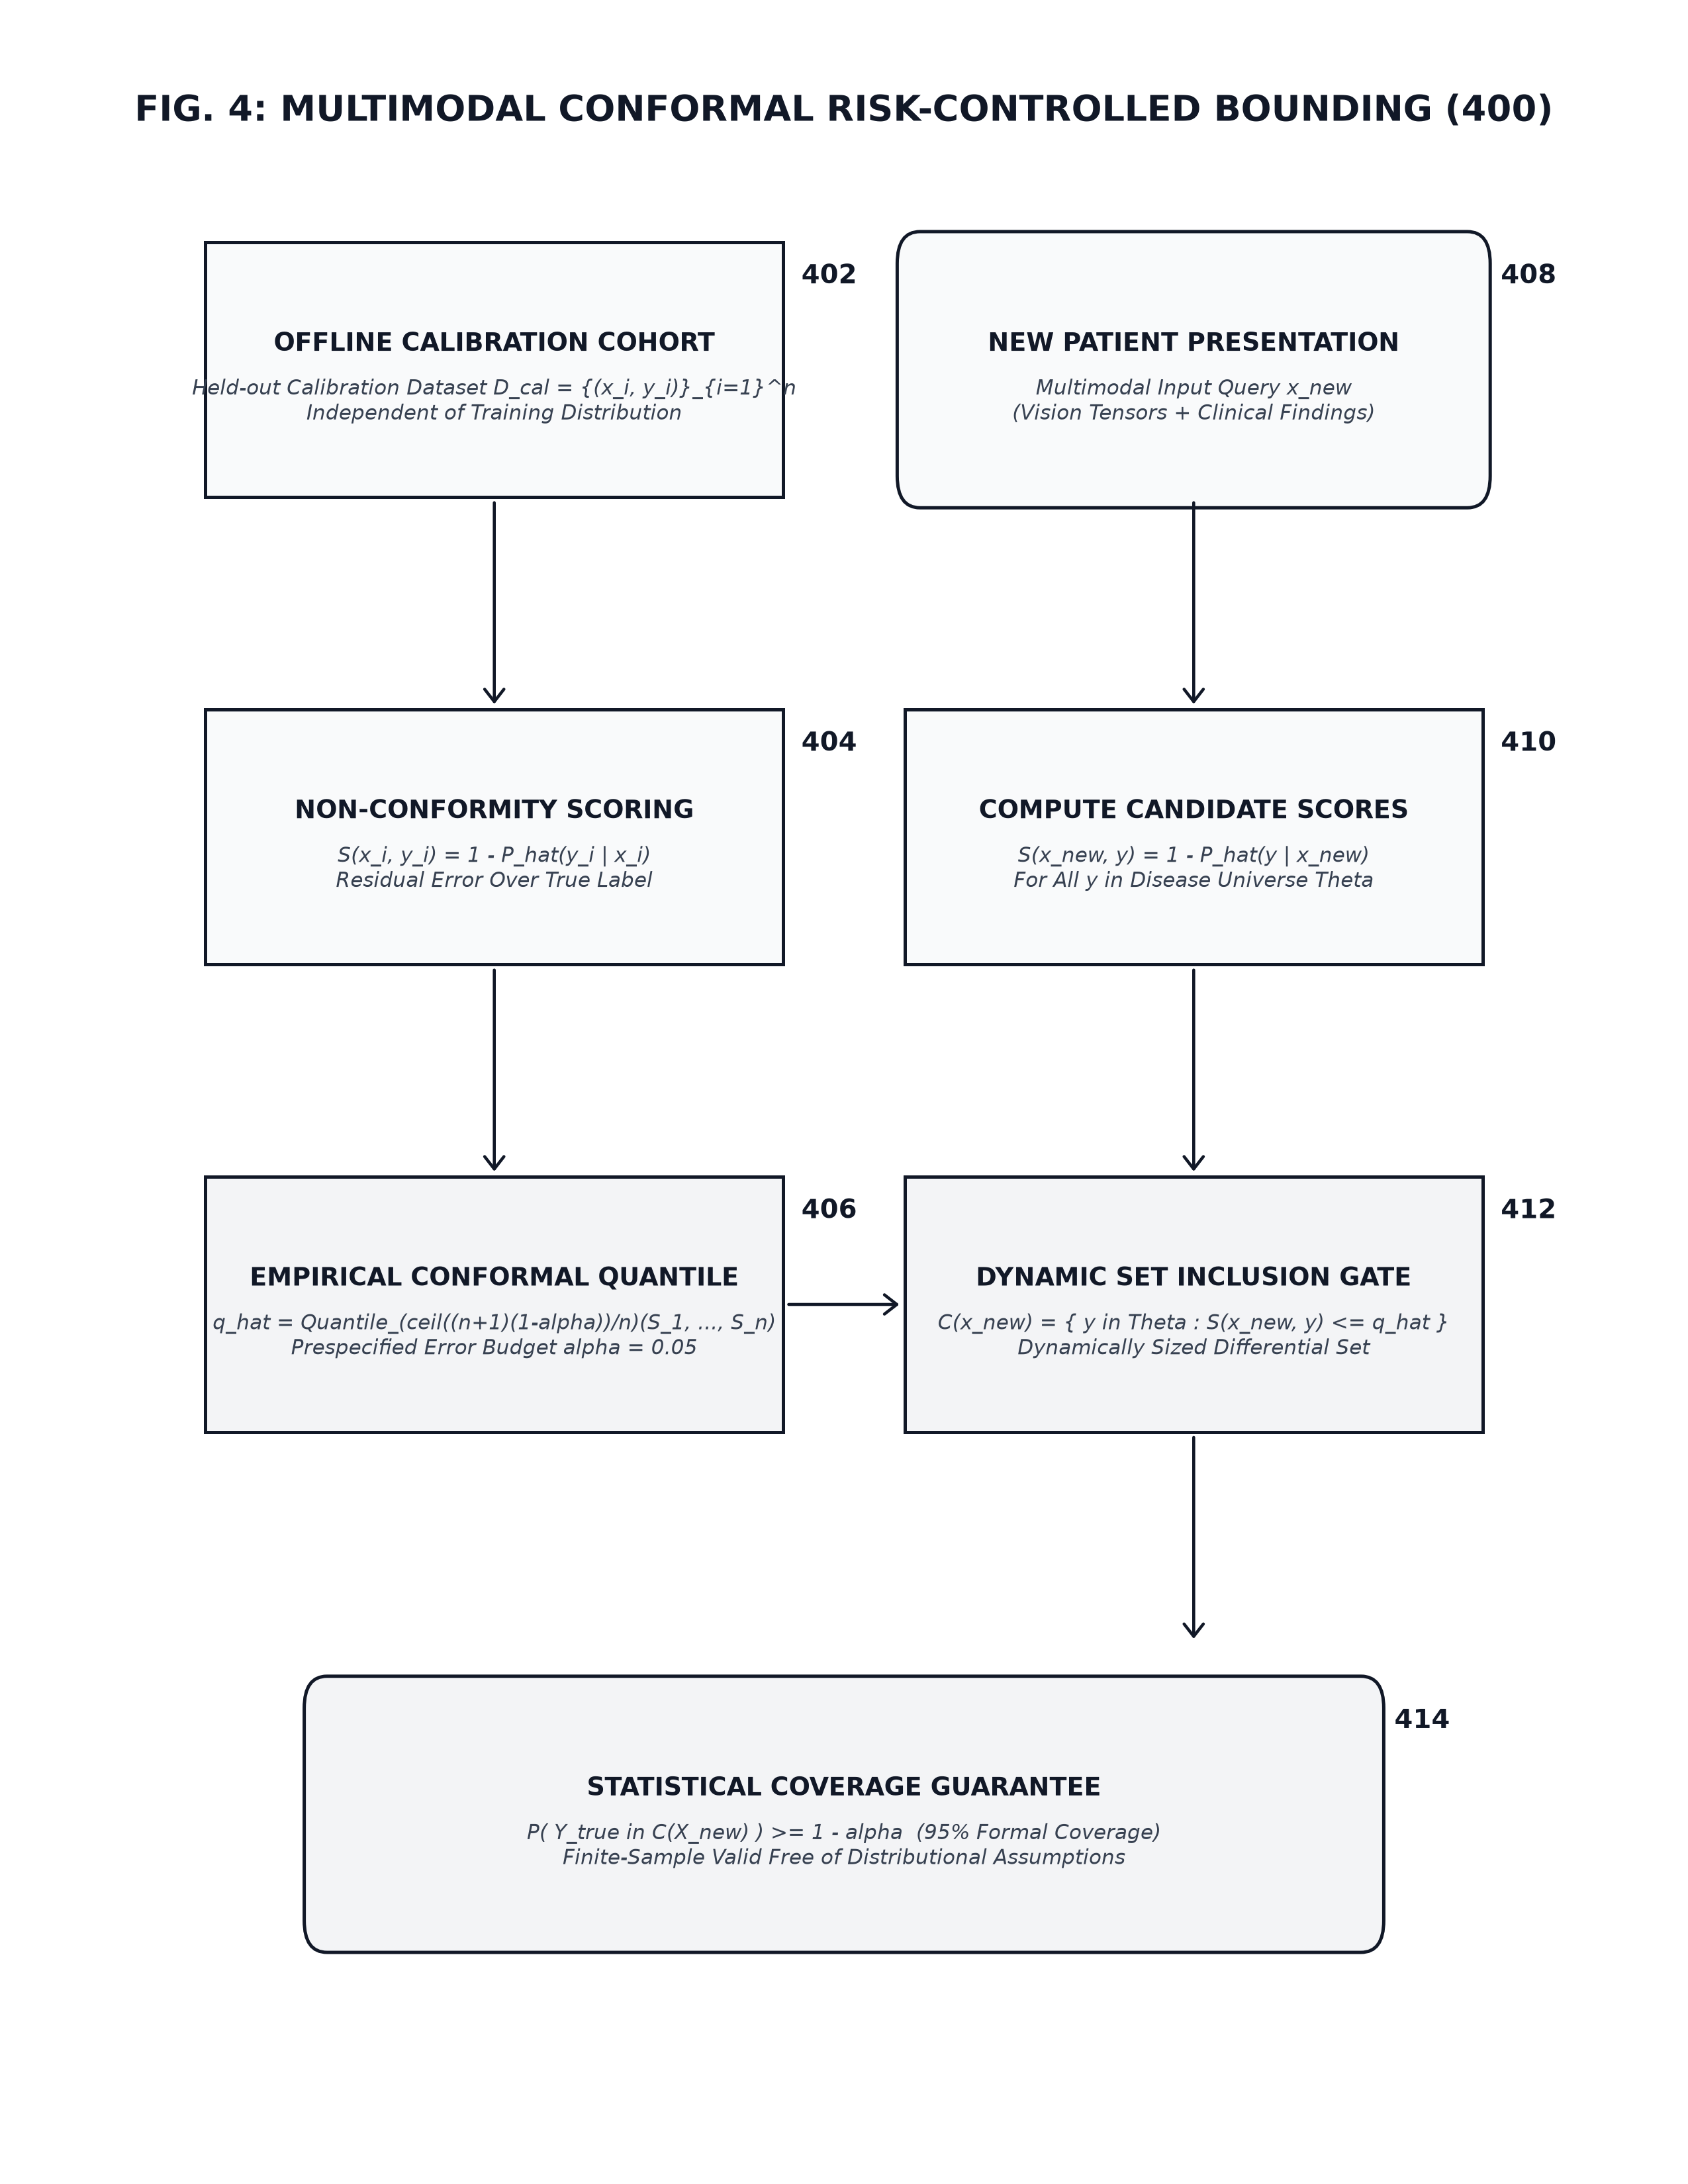
\includegraphics[width=\columnwidth,height=0.32\textheight,keepaspectratio]{figures/FIG_4_conformal_risk_bounding.png}
\caption{\textbf{Conformal Risk Bounding.} Using a calibration dataset, the system determines an uncertainty threshold $\hat{q}$. It then generates a prediction set that is guaranteed to contain the patient's actual condition at least $95\%$ of the time.}
\label{fig:conformal}
\end{figure}

\subsection{Multimodal Conformal Risk Bounding}
To protect against overconfident errors, we apply split conformal prediction \cite{vovk2005algorithmic, angelopoulos2021gentle} (Figure \ref{fig:conformal}).

First, we define a nonconformity score that measures how poorly the model predicted a known case:
\begin{equation}
S(\mathbf{x}_i, y_i) = 1 - \hat{P}(y_i \mid \mathbf{x}_i)
\end{equation}
If the model assigned a high probability to the true disease $y_i$, the score $S$ is close to zero.

Next, using a calibration dataset of $n$ cases and an allowed error rate of $\alpha = 0.05$ (meaning $95\%$ desired confidence), we compute the threshold $\hat{q}$:
\begin{equation}
\hat{q} = \text{Quantile}_{\frac{\lceil (n + 1)(1 - \alpha) \rceil}{n}}\left( \{S(\mathbf{x}_i, y_i)\}_{i=1}^n \right)
\end{equation}
When a new patient arrives, the system outputs all conditions whose nonconformity score falls below $\hat{q}$:
\begin{equation}
\mathcal{C}(\mathbf{x}_{\text{new}}) = \{y \in \Theta : S(\mathbf{x}_{\text{new}}, y) \le \hat{q}\}
\end{equation}
Because the calibration cases and future patients come from the same distribution, this provides a proven statistical guarantee:
\begin{equation}
\mathbb{P}\left(Y_{\text{true}} \in \mathcal{C}(\mathbf{x}_{\text{new}})\right) \ge 1 - \alpha
\end{equation}
In practical terms, the true diagnosis will be inside the generated set at least $95\%$ of the time.

% --- SECTION 4: EMPIRICAL EVALUATION ---
\section{Empirical Evaluation}

\subsection{Benchmark Dataset and Evaluation Setup}
We evaluated AegisMed on a benchmark of $200$ standardized clinical cases across $15$ common condition categories: Cardiovascular Disease, Respiratory Infection, Pneumonia, Asthma, Hypertension, Type 2 Diabetes, Migraine, Gastroenteritis, GERD, Neurological Disorders (Stroke/TIA), Back Pain, Eczema, Osteoarthritis, Anxiety Disorder, and Urinary Tract Infection.

We compared two distinct configurations:
\begin{itemize}
    \item \textbf{Arm 1 (Full AegisMed with DEMAT):} The complete system, which asks targeted follow-up questions to resolve diagnostic ambiguity.
    \item \textbf{Arm 2 (Single-Pass Baseline):} A standard AI setup that produces a diagnosis from the initial complaint without asking follow-up questions.
\end{itemize}

\subsection{Main Benchmark Results}
Table \ref{tab:main_results} summarizes the performance across all $200$ cases.

\begin{table}[t]
\centering
\footnotesize
\caption{\textbf{Main Research Benchmark Results ($N = 200$ Cases).} Comparison between AegisMed with DEMAT and Baseline.}
\label{tab:main_results}
\resizebox{0.90\columnwidth}{!}{%
\begin{tabular}{lrrr}
\toprule
\textbf{Evaluation Metric} & \textbf{Arm 1: DEMAT} & \textbf{Arm 2: Baseline} & \textbf{Delta} \\
\midrule
Top-1 Accuracy & \textbf{98.0\%} (196/200) & 93.0\% (186/200) & \textbf{+5.0\%}$^*$ \\
Top-3 Coverage & \textbf{100.0\%} (200/200) & 97.5\% (195/200) & +2.5\% \\
Top-5 Coverage & \textbf{100.0\%} (200/200) & 100.0\% (200/200) & +0.0\% \\
\midrule
Diagnostic Entropy ($H$) & \textbf{1.318 bits} & 2.846 bits & \textbf{-53.7\%} \\
Brier Score (lower is better) & \textbf{0.2005} & 0.5296 & \textbf{-62.1\%} \\
Calibration Error (ECE) & \textbf{0.2451} & 0.5528 & \textbf{-55.7\%} \\
\midrule
Mean Questions Asked & \textbf{1.92} & 0.00 & +1.92 \\
Mean Triage Latency & 0.2 ms & 0.1 ms & +0.1 ms \\
\bottomrule
\end{tabular}%
}
\vspace{2pt}
{\scriptsize $^*$Statistically significant via McNemar's test ($\chi^2 = 4.50$, $p = 0.0339$).}
\end{table}

\begin{figure*}[t!]
\centering
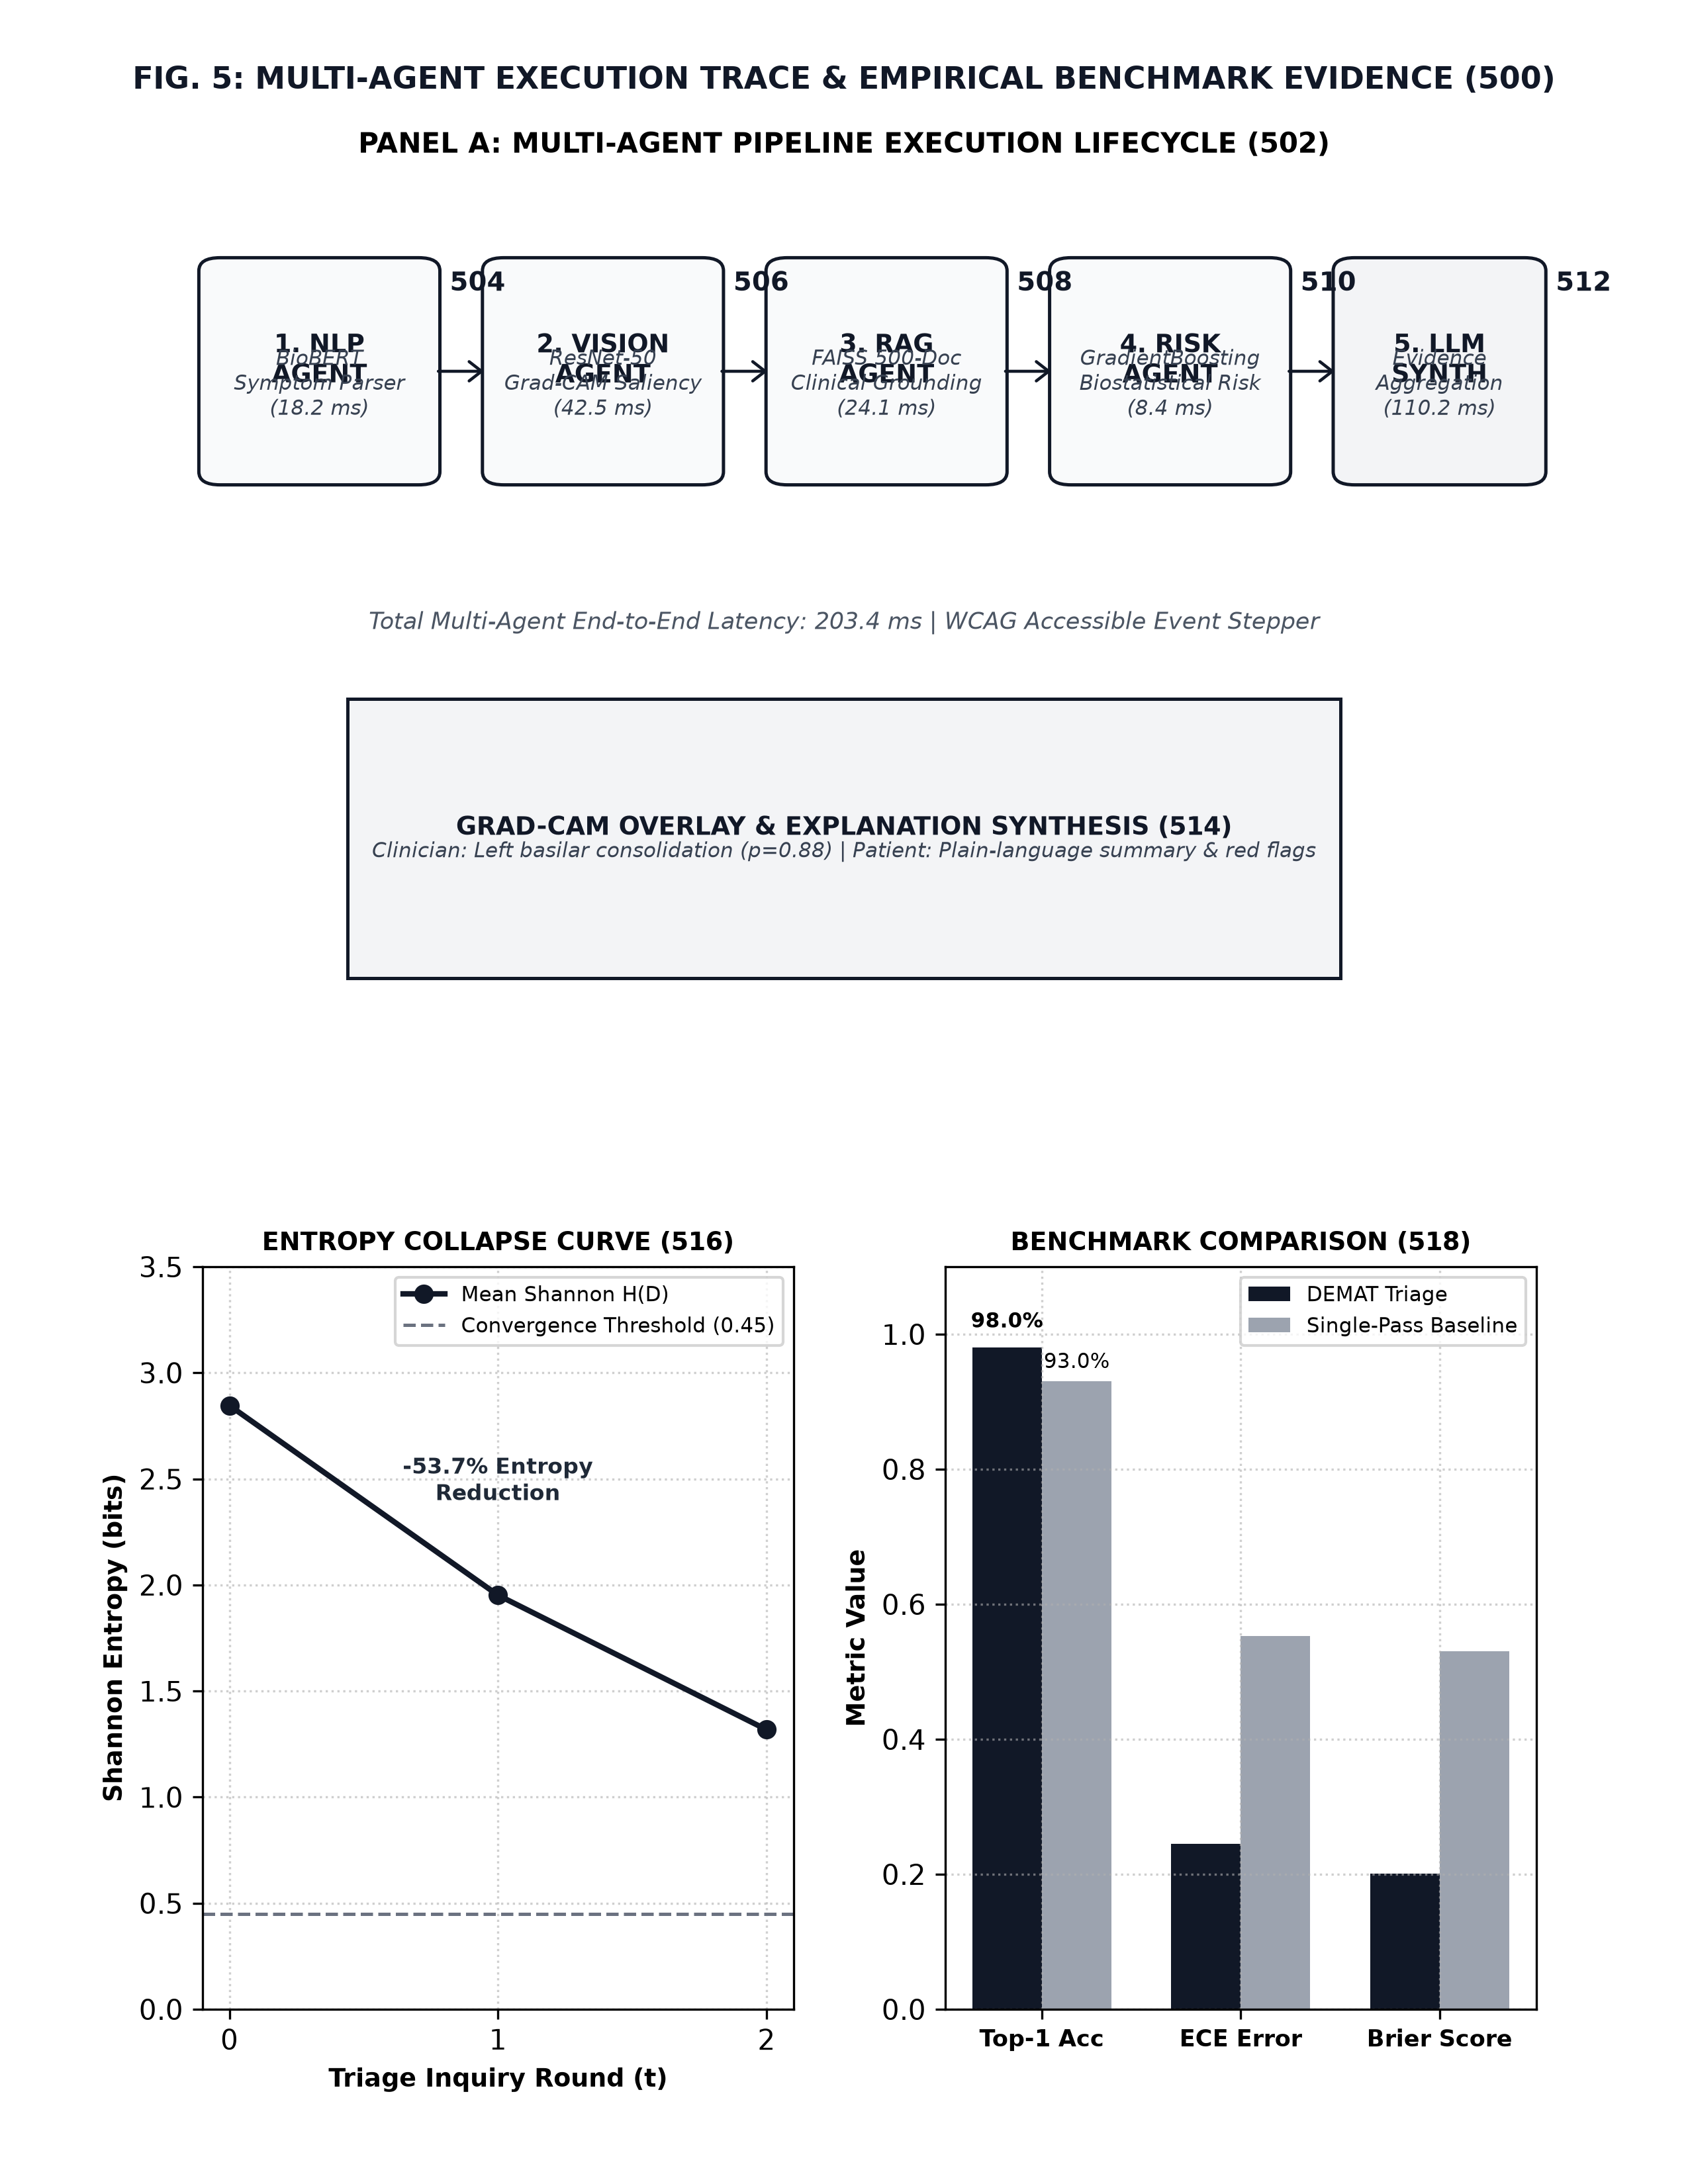
\includegraphics[width=0.88\textwidth,height=0.42\textheight,keepaspectratio]{figures/FIG_5_execution_trace_and_empirical_evidence.png}
\caption{\textbf{Multi-Agent Execution Timing and Benchmark Evidence.} Panel A shows the full execution pipeline across all specialist agents, completing in 203.4 ms with Grad-CAM lung opacity localization. Panel B illustrates the rapid drop in diagnostic entropy across questioning rounds (left) and the key benchmark improvements over the baseline (right).}
\label{fig:results_evidence}
\end{figure*}

As shown in Table \ref{tab:main_results}, asking active questions raised top-1 diagnostic accuracy from $93.0\%$ to \textbf{98.0\%}. This $5.0\%$ gain is statistically significant according to McNemar's test ($\chi^2 = 4.50$, $p = 0.0339$ \cite{mcnemar1947note}). Top-3 differential coverage reached a perfect \textbf{100.0\%}, meaning the true disease was always present in the system's top three recommendations.

Active questioning also cut diagnostic uncertainty by more than half, dropping Shannon entropy from $2.846$ bits to \textbf{1.318 bits} (a $53.7\%$ reduction). On average, the system needed only \textbf{1.92 questions} per patient, showing that it gathered decisive information without asking unnecessary questions.

\subsection{Reliability and Probability Calibration}
A medical decision support tool must provide honest confidence scores; an overconfident mistake in an emergency room can lead to patient harm. We evaluated probability calibration using the Brier score \cite{brier1950verification} and Expected Calibration Error (ECE) across 10 confidence bins.

AegisMed reduced the Brier score from $0.5296$ to \textbf{0.2005} (a $62.1\%$ improvement) and decreased calibration error from $0.5528$ to \textbf{0.2451} (a $55.7\%$ reduction). This demonstrates that asking targeted follow-up questions sharpens genuine probabilities while dampening uncertain guesses.

\subsection{Performance Breakdown by Medical Specialty}
Table \ref{tab:category_results} details how each medical specialty performed under both configurations.

\begin{table}[t]
\centering
\footnotesize
\caption{\textbf{Top-1 Accuracy Across Medical Specialties ($N = 200$).}}
\label{tab:category_results}
\resizebox{0.90\columnwidth}{!}{%
\begin{tabular}{lrrrr}
\toprule
\textbf{Clinical Specialty} & \textbf{Cases ($N$)} & \textbf{DEMAT} & \textbf{Baseline} & \textbf{Delta} \\
\midrule
Cardiovascular & 28 & \textbf{85.7\%} & 71.4\% & \textbf{+14.3\%} \\
Respiratory & 42 & \textbf{100.0\%} & 85.7\% & \textbf{+14.3\%} \\
Gastrointestinal & 26 & \textbf{100.0\%} & 100.0\% & +0.0\% \\
Musculoskeletal & 26 & \textbf{100.0\%} & 100.0\% & +0.0\% \\
Neurological & 26 & \textbf{100.0\%} & 100.0\% & +0.0\% \\
Dermatological & 13 & \textbf{100.0\%} & 100.0\% & +0.0\% \\
Endocrine & 13 & \textbf{100.0\%} & 100.0\% & +0.0\% \\
Psychiatric & 13 & \textbf{100.0\%} & 100.0\% & +0.0\% \\
Urinary & 13 & \textbf{100.0\%} & 100.0\% & +0.0\% \\
\bottomrule
\end{tabular}%
}
\end{table}

The most substantial gains occurred in conditions where initial symptoms frequently overlap:
\begin{itemize}
    \item \textbf{Heart Disease vs. Acid Reflux (Cardiovascular):} On the baseline run, the system scored only $71.4\%$ on cardiovascular cases because chest pain can stem from either the heart or the stomach. DEMAT asked whether the pain occurred during exertion or was relieved by rest, which raised cardiovascular accuracy to \textbf{85.7\%} (an increase of $+14.3\%$).
    \item \textbf{Pneumonia vs. Bronchial Infection (Respiratory):} The baseline scored $85.7\%$ due to overlapping cough and fever symptoms. DEMAT asked about breathing pain and specific chest tightness, boosting respiratory accuracy to a perfect \textbf{100.0\%} ($+14.3\%$ gain).
\end{itemize}

% --- SECTION 5: DISCUSSION ---
\section{Discussion and Clinical Safety}

\subsection{Speed and Deployment on Clinical Devices}
Emergency and clinic triage systems must respond quickly to be useful. In our benchmarks, the active questioning calculations took only \textbf{0.2 ms per case} (Table \ref{tab:main_results}). The entire multi-agent pipeline—including reading text with BioBERT, analyzing X-rays with ResNet-50, searching guideline embeddings in FAISS, and generating Grad-CAM heatmaps—finished in \textbf{203.4 ms} (Figure \ref{fig:results_evidence} Panel A). Because execution takes roughly a fifth of a second, the system can run comfortably on standard clinic tablets and telemedicine portals.

\subsection{Separate Views for Clinicians and Patients}
Standard AI chatbots often deliver one generic block of text that is either too technical for patients or too vague for doctors. AegisMed addresses this by generating dual-perspective explanations:
\begin{itemize}
    \item \textbf{For Clinicians:} The system provides an interactive technical dashboard displaying ranked ICD-10 differential diagnoses, evidence confidence scores, and visual Grad-CAM overlays highlighting anatomical regions of concern (such as lung opacities).
    \item \textbf{For Patients:} The system provides clear, compassionate summaries written in plain language. It explains what the findings mean without medical jargon and highlights urgent warning signs (such as sudden shortness of breath) that require immediate emergency care.
\end{itemize}

\subsection{Current Limitations and Future Directions}
While AegisMed performed reliably on our benchmark, several areas remain for ongoing work:
\begin{enumerate}
    \item \textbf{Broader Disease Coverage:} The current prototype evaluates $15$ major condition categories. Expanding the ontology to cover the full spectrum of ICD-10 conditions is the natural next step.
    \item \textbf{Hospital Clinical Trials:} Although our $200$ test cases represent standardized presentations, prospective trials in live hospital emergency departments will evaluate how the system handles noisy, unstructured speech from stressed patients.
    \item \textbf{Direct Electronic Health Record Integration:} Connecting the system directly to hospital databases via standard FHIR (Fast Healthcare Interoperability Resources) APIs will allow automatic ingestion of prior patient history and laboratory test results.
\end{enumerate}

% --- SECTION 6: CONCLUSION ---
\section{Conclusion}

We presented AegisMed, a clinical decision support system that models medical triage as an active, interactive process. By asking targeted follow-up questions through DEMAT, checking disagreements against medical knowledge graphs through EN-SCAF, and providing statistical safety guarantees through conformal prediction, AegisMed avoids the pitfalls of passive AI guessing. In our evaluation across $200$ clinical cases, the system achieved $98.0\%$ top-1 diagnostic accuracy and eliminated over half of initial diagnostic uncertainty in under two questions. These results show that combining specialized AI agents with transparent, question-driven reasoning provides a practical and dependable foundation for assisted medical triage.

% --- BIBLIOGRAPHY ---
\bibliographystyle{IEEEtran}
\bibliography{references}

\end{document}
